\section{Data Preprocessing}
    \subsection{Small Stack}
        \begin{figure}[H]
            \centering
            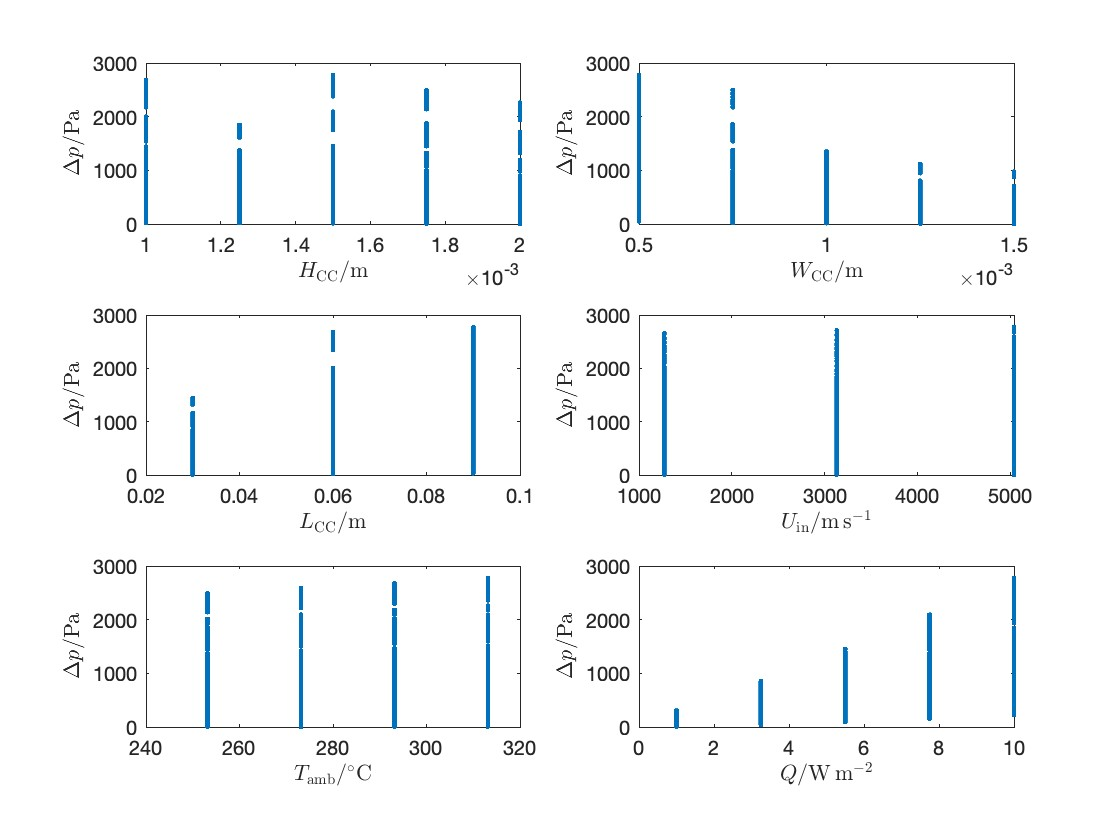
\includegraphics[width=1\textwidth]{00_Images/00_Small_Stack_Images/00_Pressure_Drop_vs_Features_July_10_2024_v1.jpg}  % Change "example-image" to the filename of your image
            \caption{This is an example image.}
            \label{fig:example1}
        \end{figure}

        \begin{figure}[H]
            \centering
            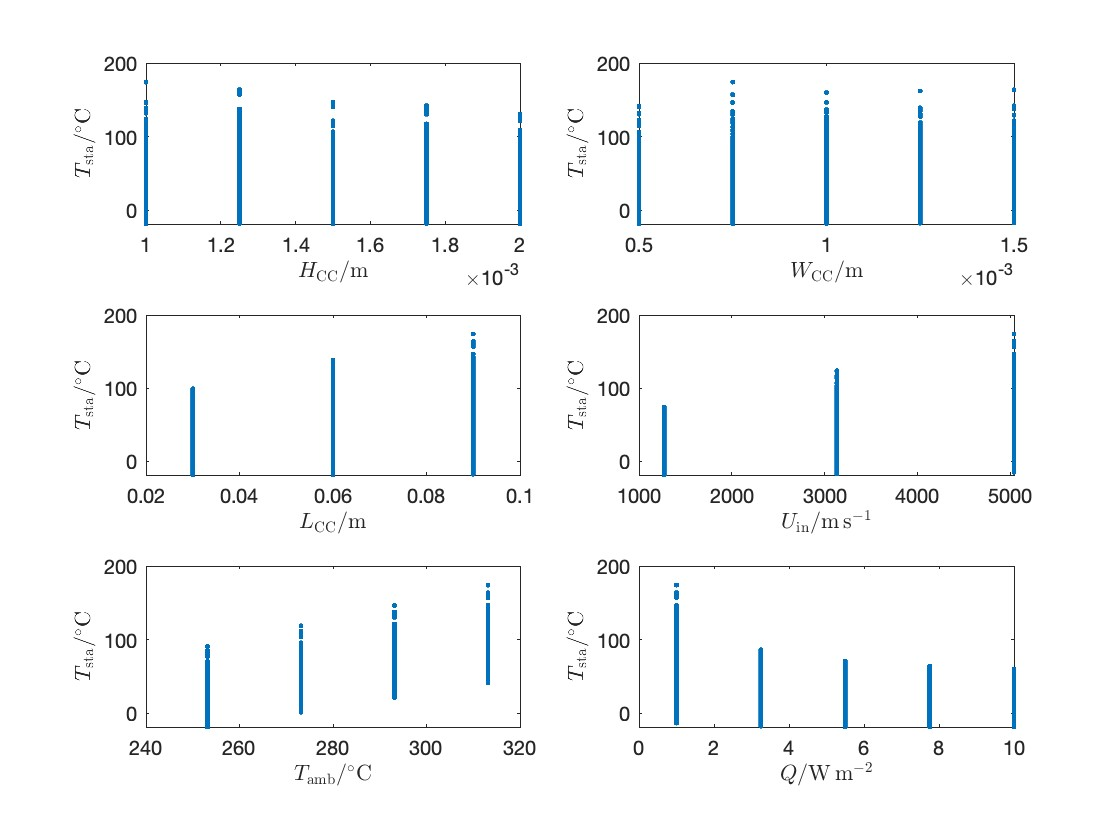
\includegraphics[width=1\textwidth]{00_Images/00_Small_Stack_Images/00_Temperature_vs_Features_July_10_2024_v1.jpg}  % Change "example-image" to the filename of your image
            \caption{This is an example image.}
            \label{fig:example1}
        \end{figure}

        \begin{figure}[H]
            \centering
            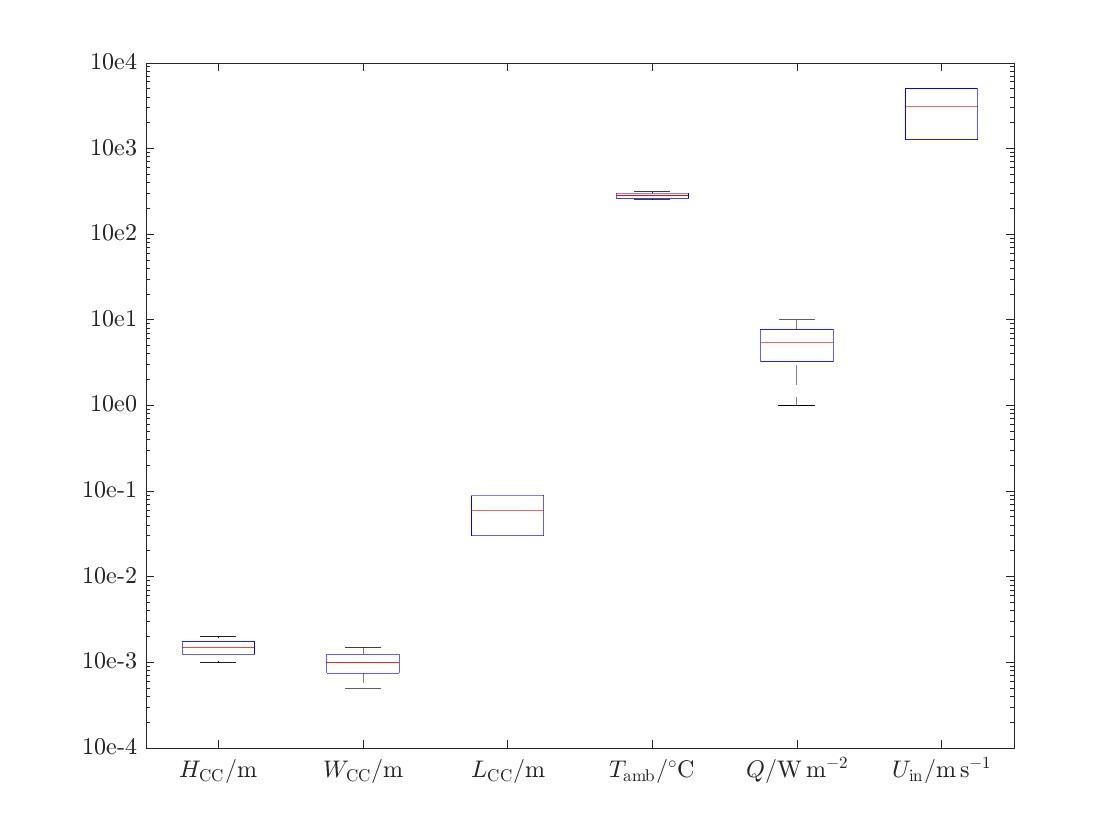
\includegraphics[width=1\textwidth]{00_Images/00_Small_Stack_Images/00_Combined_Boxplot_Features_July_10_2024_v1.jpg}  % Change "example-image" to the filename of your image
            \caption{This is an example image.}
            \label{fig:example1}
        \end{figure}

        \begin{figure}[H]
            \centering
            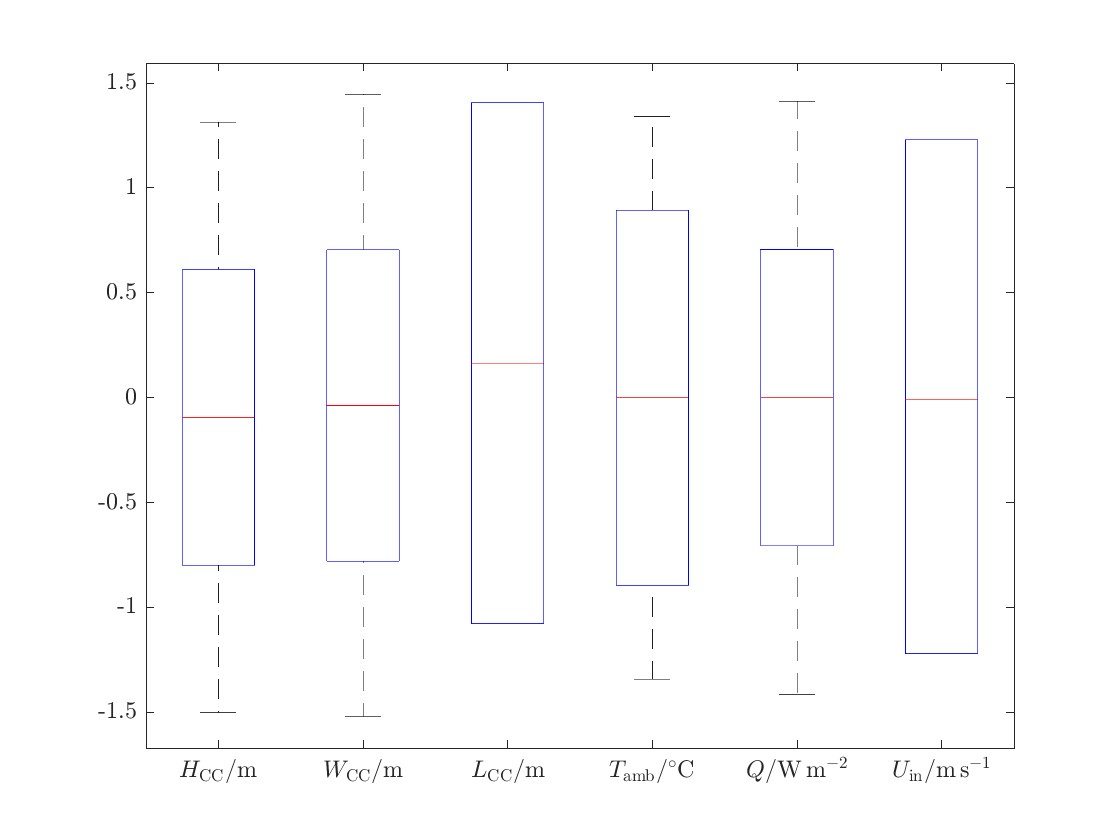
\includegraphics[width=1\textwidth]{00_Images/00_Small_Stack_Images/00_Combined_Boxplot_Normalized_Features_July_10_2024_v1.jpg}  % Change "example-image" to the filename of your image
            \caption{This is an example image.}
            \label{fig:example1}
        \end{figure}

        \begin{figure}[H]
            \centering
            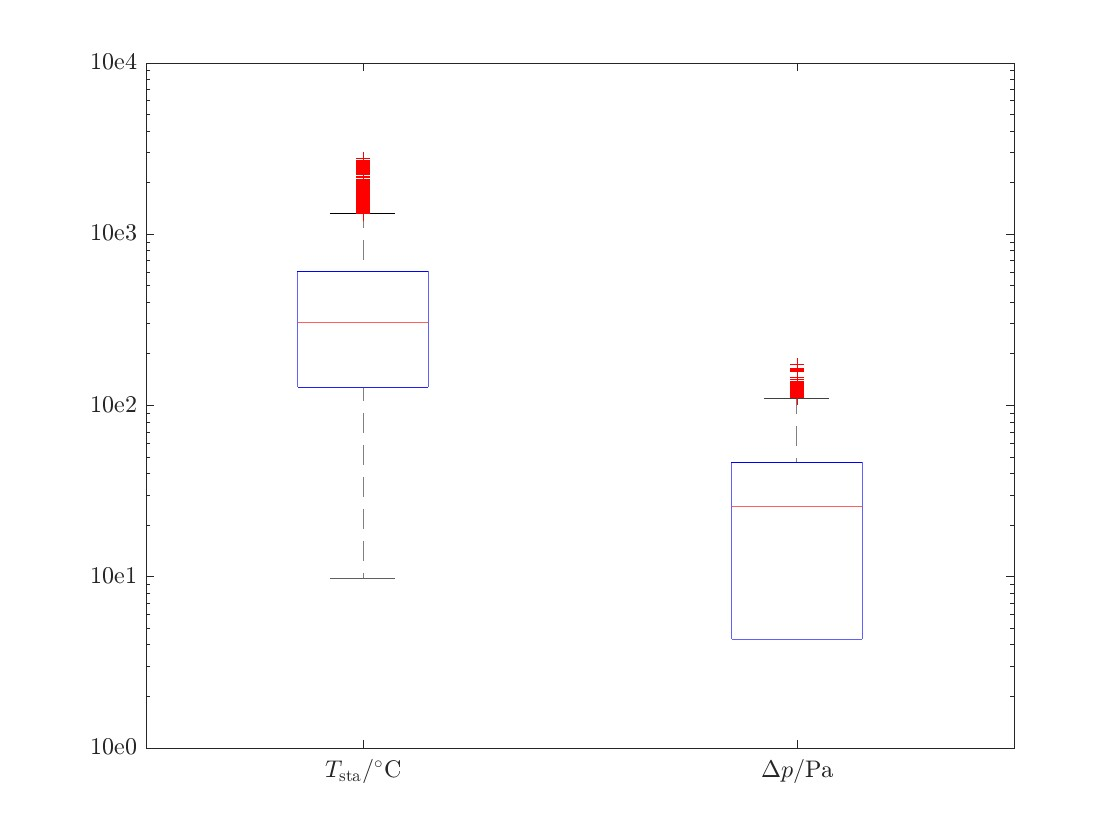
\includegraphics[width=1\textwidth]{00_Images/00_Small_Stack_Images/00_Combined_Boxplot_Outputs_July_10_2024_v1.jpg}  % Change "example-image" to the filename of your image
            \caption{This is an example image.}
            \label{fig:example1}
        \end{figure}

        \begin{figure}[H]
            \centering
            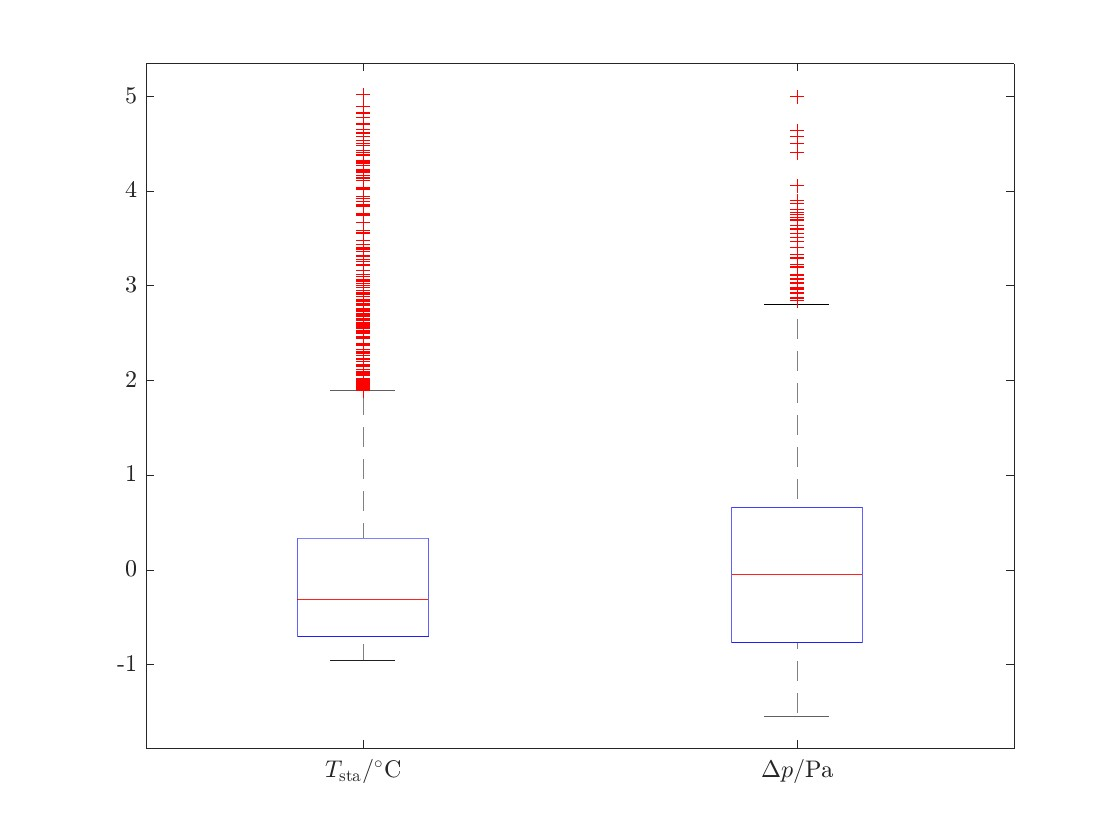
\includegraphics[width=1\textwidth]{00_Images/00_Small_Stack_Images/00_Combined_Boxplot_Normalized_Outputs_July_10_2024_v1.jpg}  % Change "example-image" to the filename of your image
            \caption{This is an example image.}
            \label{fig:example1}
        \end{figure}

        \begin{figure}[H]
            \centering
            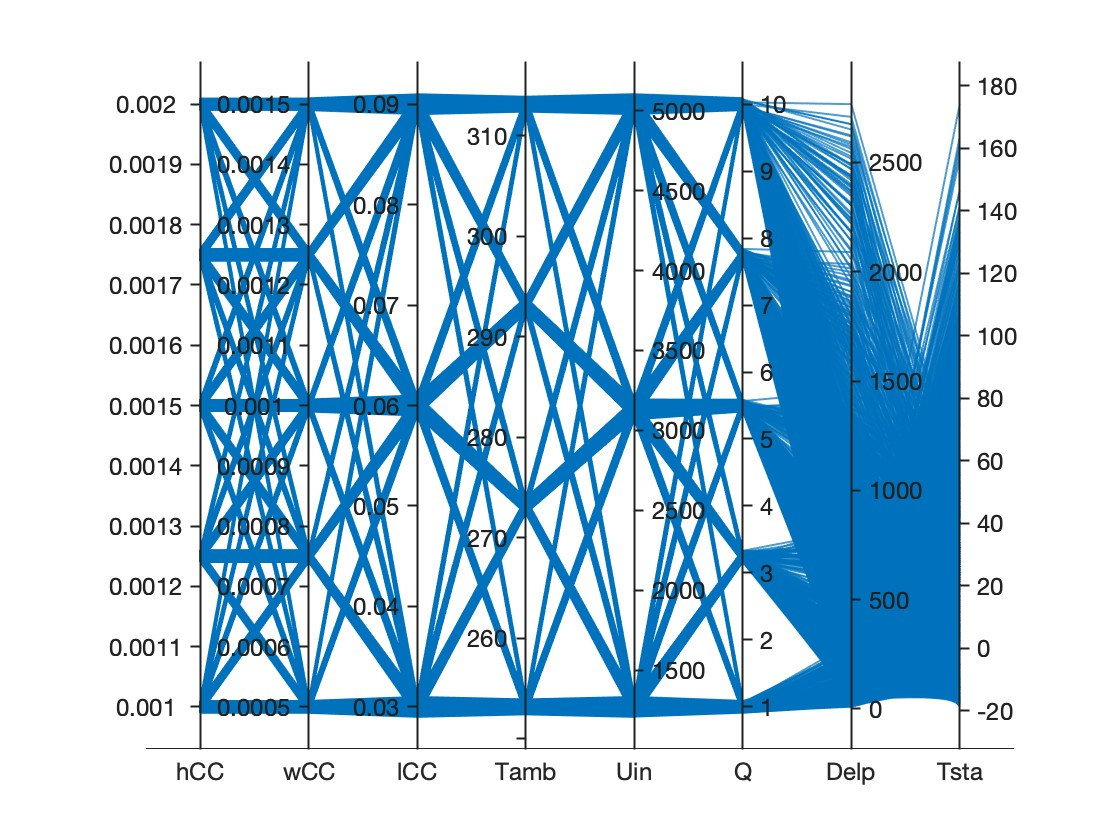
\includegraphics[width=1\textwidth]{00_Images/00_Small_Stack_Images/00_Parallel_Coordinate_Plot_July_10_2024_v1.jpg}  % Change "example-image" to the filename of your image
            \caption{This is an example image.}
            \label{fig:example1}
        \end{figure}

        \begin{figure}[H]
            \centering
            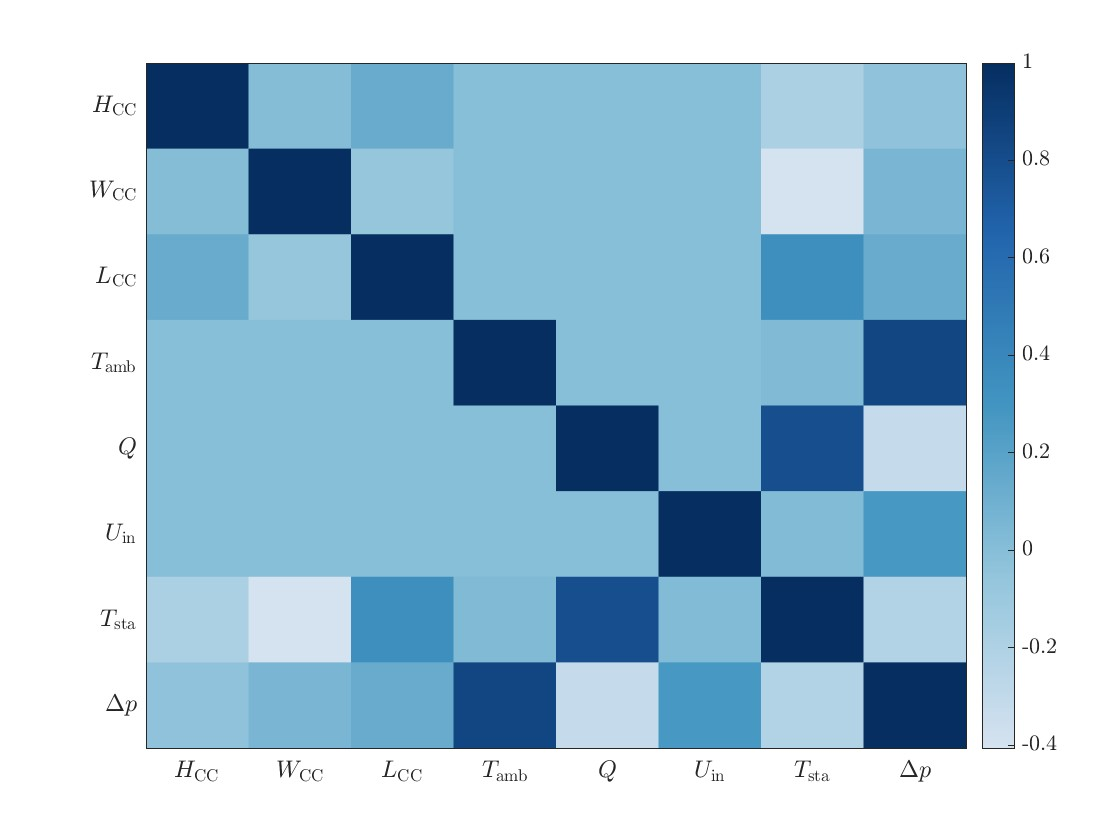
\includegraphics[width=1\textwidth]{00_Images/00_Small_Stack_Images/00_Spearman_Correlation_Matrix_Heatmap_July_10_2024_v1.jpg}  % Change "example-image" to the filename of your image
            \caption{This is an example image.}
            \label{fig:example1}
        \end{figure}

    \subsection{Large Stack}
        \begin{figure}[H]
            \centering
            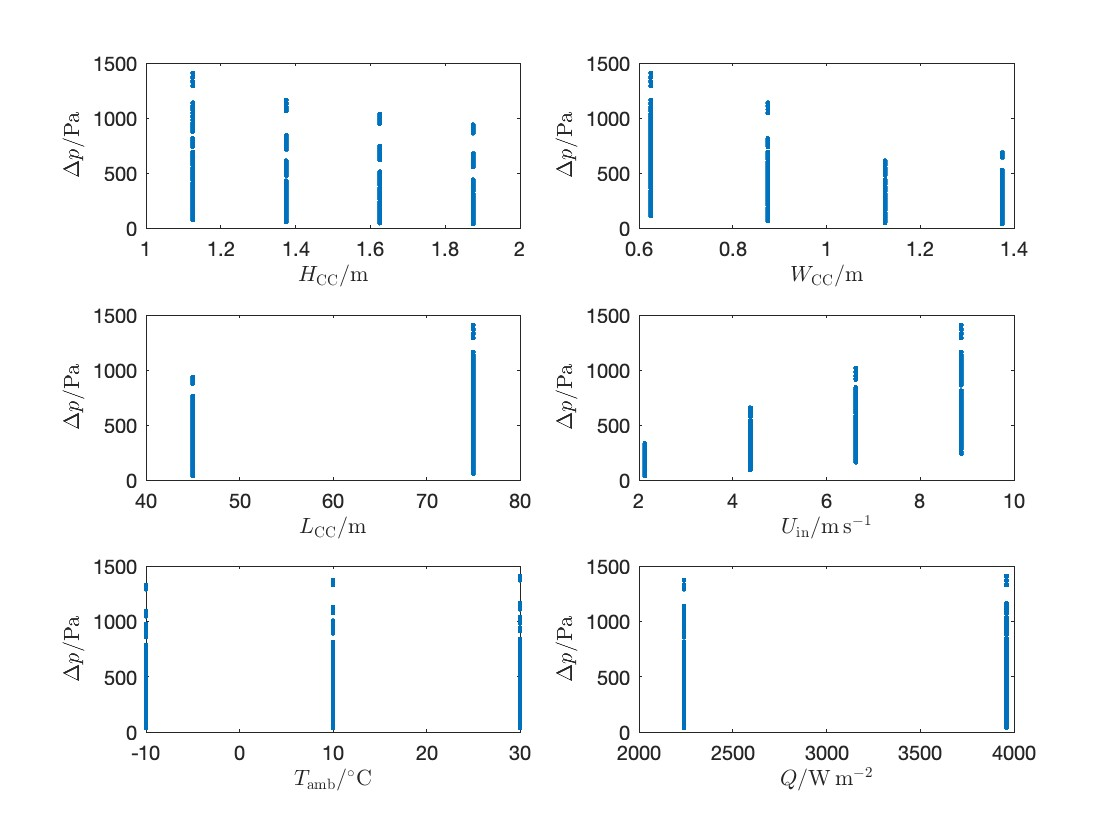
\includegraphics[width=1\textwidth]{00_Images/00_Large_Stack_Images/00_Pressure_Drop_vs_Features_July_10_2024_v1.jpg}  % Change "example-image" to the filename of your image
            \caption{This is an example image.}
            \label{fig:example1}
        \end{figure}

        \begin{figure}[H]
            \centering
            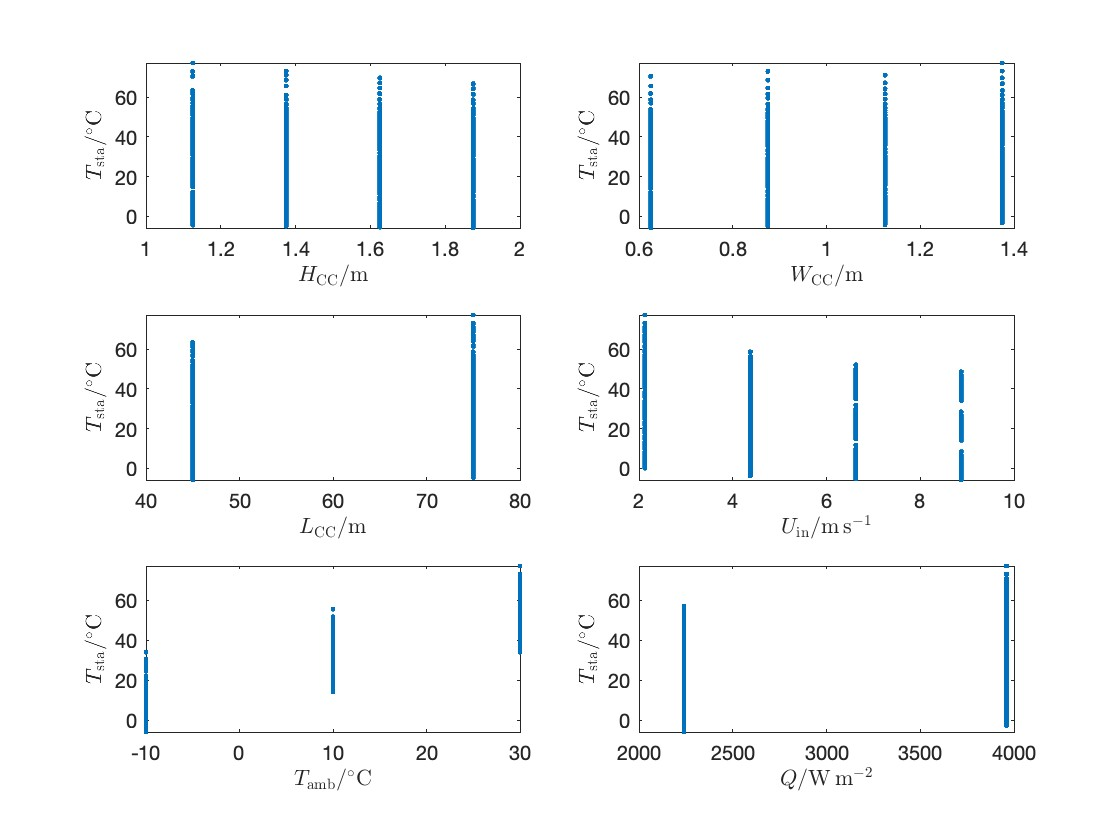
\includegraphics[width=1\textwidth]{00_Images/00_Large_Stack_Images/00_Temperature_vs_Features_July_10_2024_v1.jpg}  % Change "example-image" to the filename of your image
            \caption{This is an example image.}
            \label{fig:example1}
        \end{figure}

        \begin{figure}[H]
            \centering
            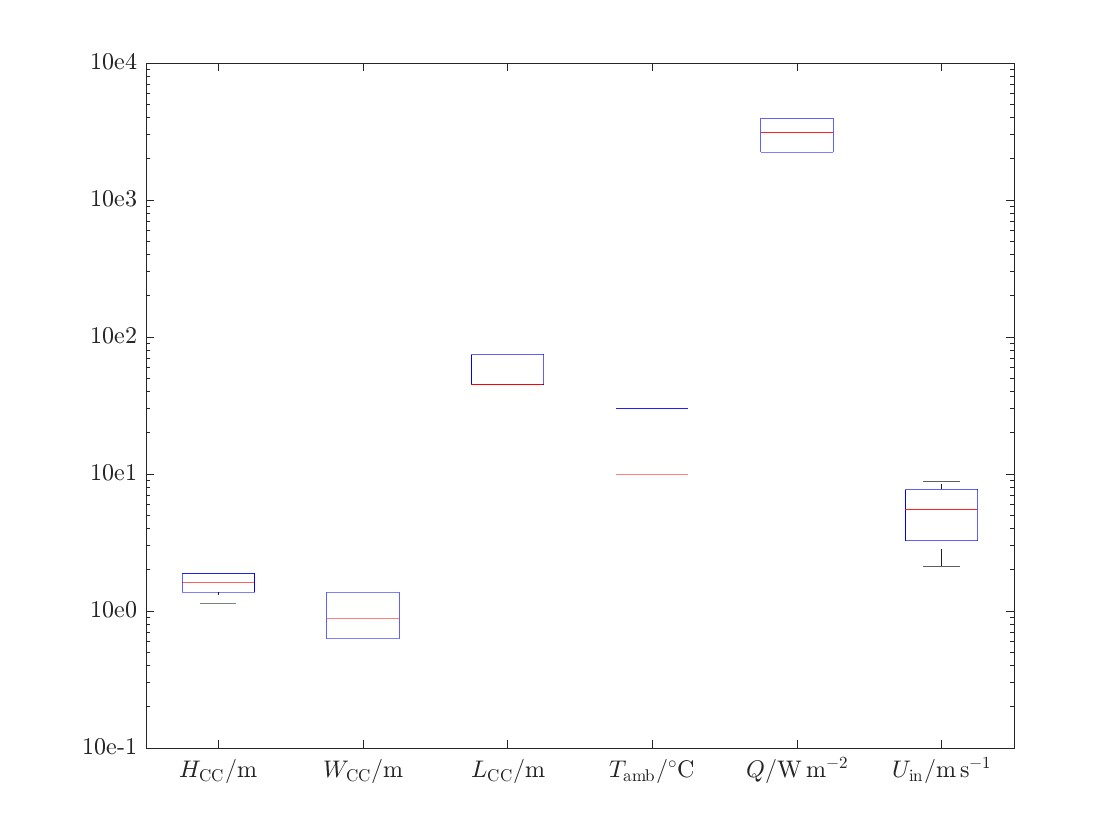
\includegraphics[width=1\textwidth]{00_Images/00_Large_Stack_Images/00_Combined_Boxplot_Features_July_10_2024_v1.jpg}  % Change "example-image" to the filename of your image
            \caption{This is an example image.}
            \label{fig:example1}
        \end{figure}

        \begin{figure}[H]
            \centering
            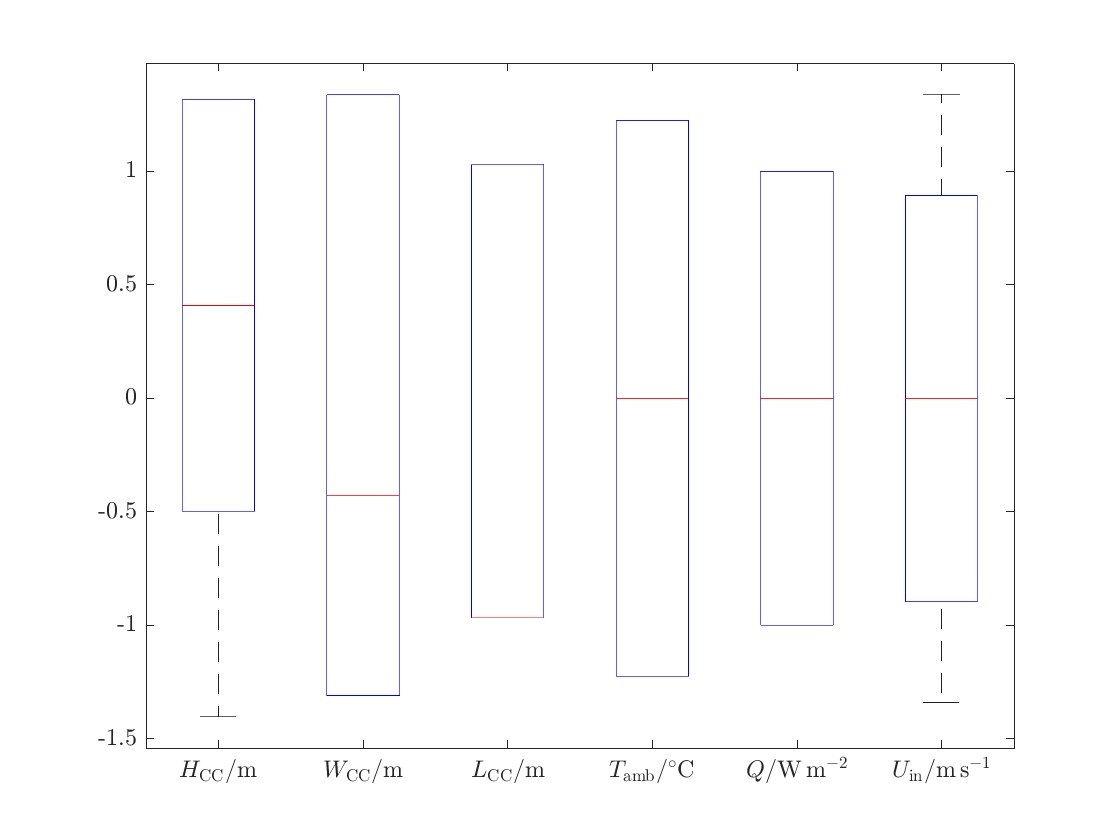
\includegraphics[width=1\textwidth]{00_Images/00_Large_Stack_Images/00_Combined_Boxplot_Normalized_Features_July_10_2024_v1.jpg}  % Change "example-image" to the filename of your image
            \caption{This is an example image.}
            \label{fig:example1}
        \end{figure}

        \begin{figure}[H]
            \centering
            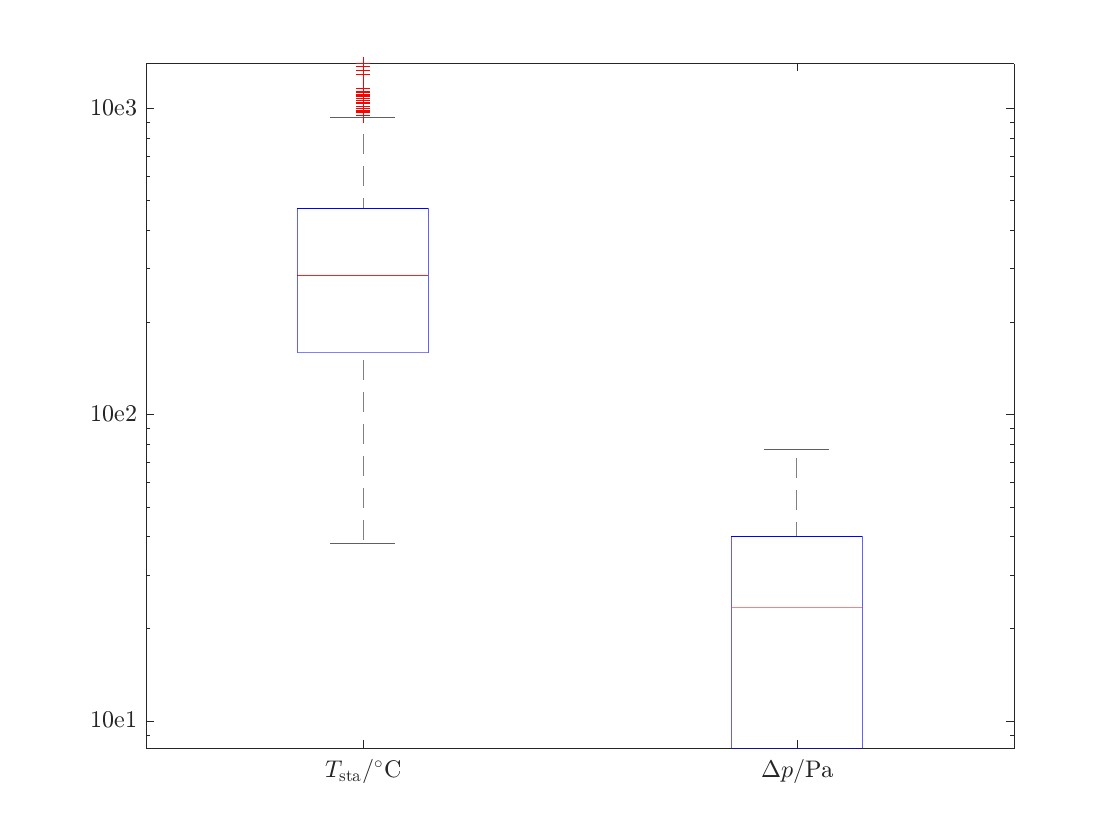
\includegraphics[width=1\textwidth]{00_Images/00_Large_Stack_Images/00_Combined_Boxplot_Outputs_July_10_2024_v1.jpg}  % Change "example-image" to the filename of your image
            \caption{This is an example image.}
            \label{fig:example1}
        \end{figure}

        \begin{figure}[H]
            \centering
            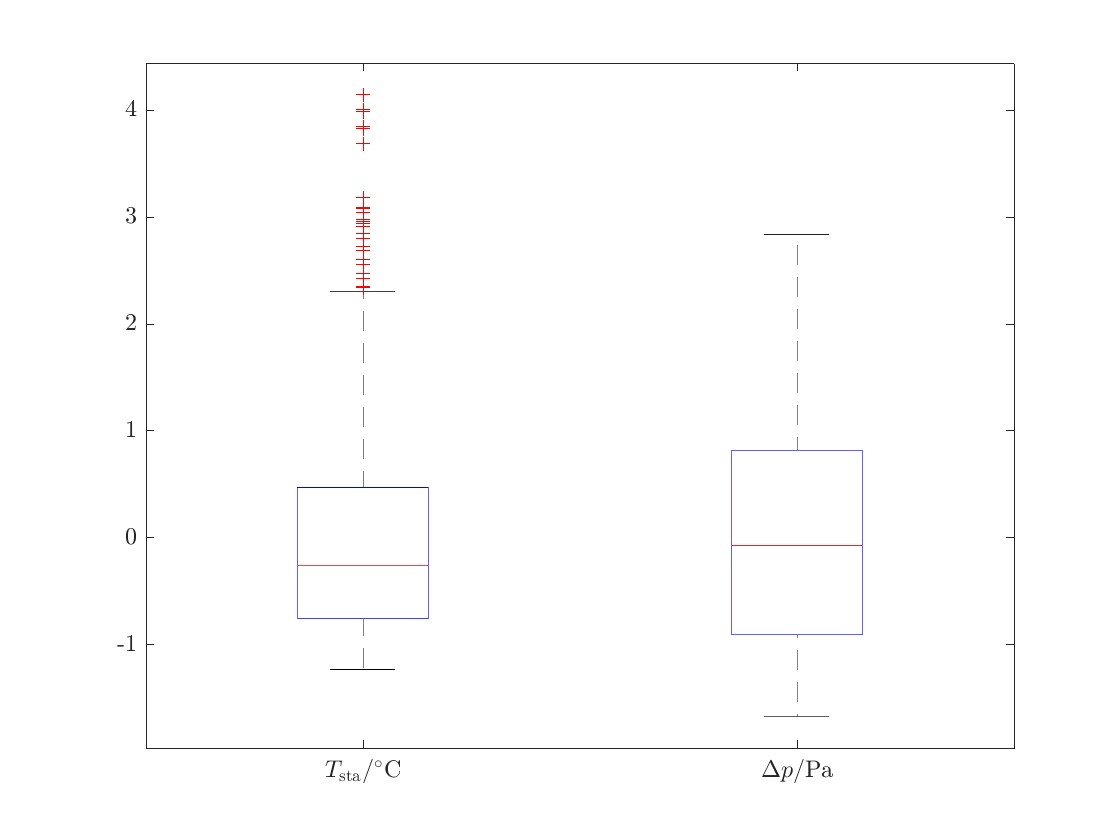
\includegraphics[width=1\textwidth]{00_Images/00_Large_Stack_Images/00_Combined_Boxplot_Normalized_Outputs_July_10_2024_v1.jpg}  % Change "example-image" to the filename of your image
            \caption{This is an example image.}
            \label{fig:example1}
        \end{figure}

        \begin{figure}[H]
            \centering
            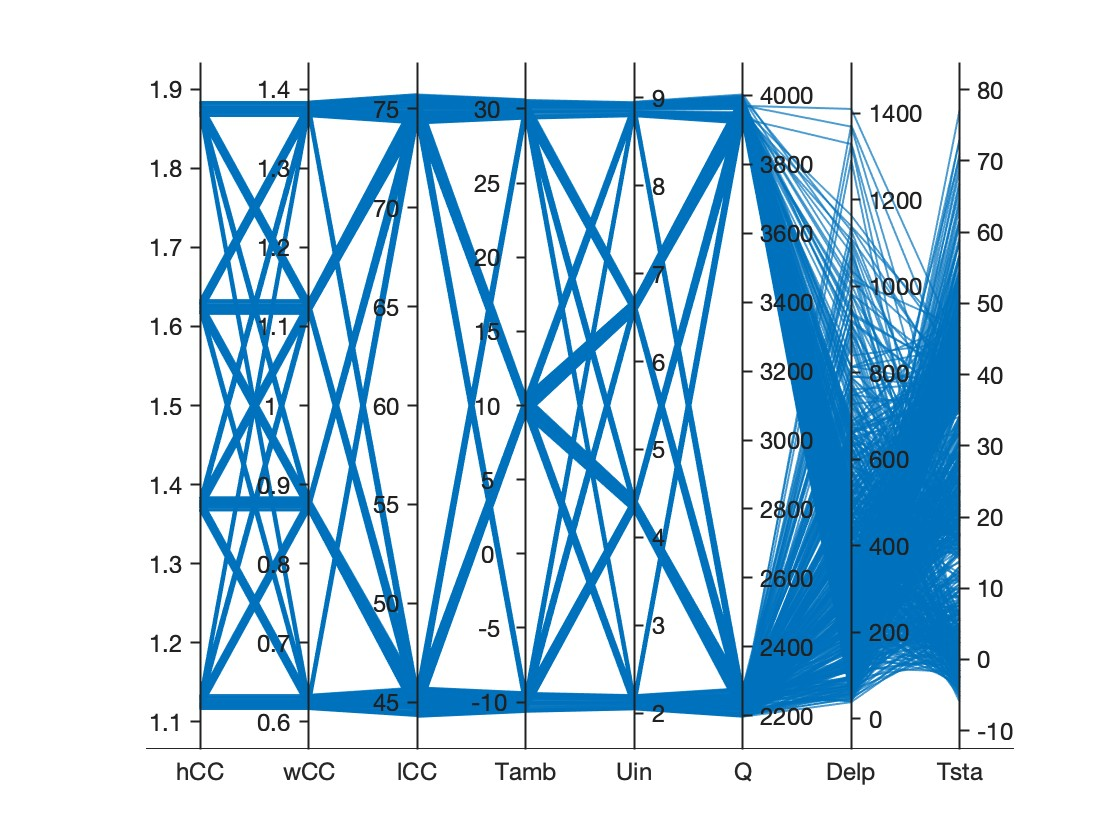
\includegraphics[width=1\textwidth]{00_Images/00_Large_Stack_Images/00_Parallel_Coordinate_Plot_July_10_2024_v1.jpg}  % Change "example-image" to the filename of your image
            \caption{This is an example image.}
            \label{fig:example1}
        \end{figure}

        \begin{figure}[H]
            \centering
            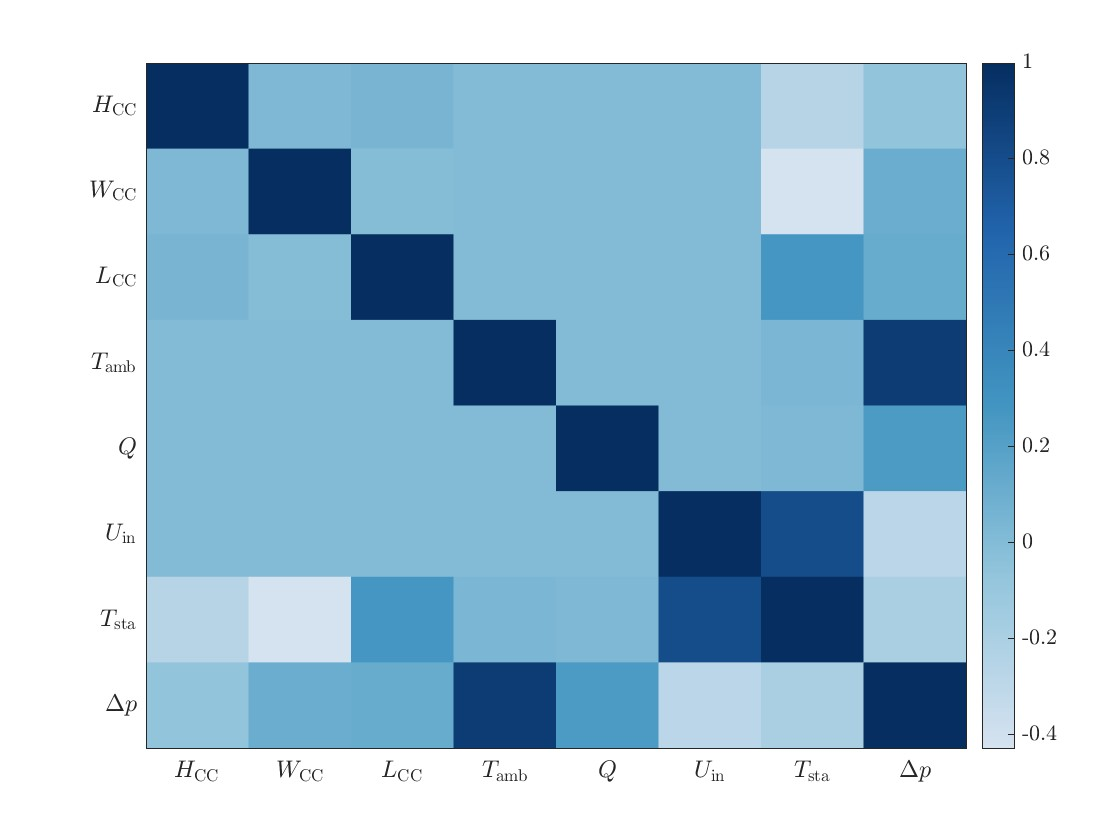
\includegraphics[width=1\textwidth]{00_Images/00_Large_Stack_Images/00_Spearman_Correlation_Matrix_Heatmap_July_10_2024_v1.jpg}  % Change "example-image" to the filename of your image
            \caption{This is an example image.}
            \label{fig:example1}
        \end{figure}

            